
\centerline{\textbf{ \LARGE Paging}}


% ----------------------------------------------------------------------------


\begin{enumerate}

  \begin{figure}[h]
      \centering   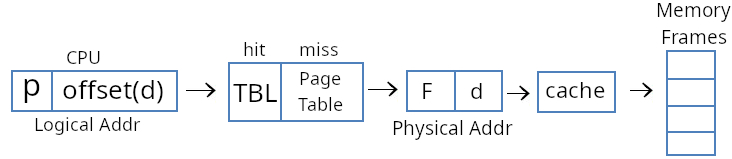
\includegraphics[scale=2.5]{./images/paging_01.jpeg}
  \end{figure}
  \item Paging \\
  \begin{myTableStyle}
    \begin{tabular}{ |m{3.5cm}|m{10cm}| } \hline
        Frame           &     Physical Address Space divided into frames                  \\ \hline
        Page            &     Logical   Address Space divided into pages.                 \\
                        &     Page size defined by hardware                               \\ \hline
        Page Table      &     maping of page no to frame no                               \\ \hline
        Word            &     Page Size = Frame Size =  \(2^k\) words                     \\ \hline
        offset(k-bits)  &     index of the word in a page/frame  \\ \hline
        Logical address &     page no(p)  +  offset(d)                                    \\ \hline
        Physical address&     frame no(f) +  offset(d)                                    \\ \hline
        Page Table Size &     \(2^p\) x size of one entry                                       \\
                        &     \(2^p\) = No of entries in page table = total pages                \\ \hline
        Translation \mbox{Lookaside} Buffer(TLB) & Acts as cache for page table                    \\ \hline
        Page Table Base \mbox{ Register} &                                                        \\ \hline
    \end{tabular}
  \end{myTableStyle}
  \vspace{0.08in}

  \item Each process has a page table.
  \item PT can not be in registers because registers are small in size.
  \item PT are kept in memory. Two main memory references are required to access a word in memory.
  \item Page table entry (PTE) \\
  \begin{myTableStyle}
    \begin{tabular}{ |m{2cm}|m{2cm}|m{2cm}|m{2cm}|m{3cm}| } \hline
        Page no &  Frame no & Valid bit & Dirty bit & Protection bit  \\ \hline
    \end{tabular}
  \end{myTableStyle}
  \vspace{0.08in}


  \item TLB : https://www.geeksforgeeks.org/translation-lookaside-buffer-tlb-in-paging/
    \begin{enumerate}
      \item Is a high-speed cache that stores a part of page table(PT).
      \item TLB miss : TLB is updated with new PTE.
      \item TLB entry replacement policies : FIFO, LRU or MFU etc
      \item TLB first checks. If the page is not in memory a page fault is issued then the TLB is updated to include the new page entry.
    \end{enumerate}
    \vspace{0.08in}

    \item Page sharing : multiple processes share the same  frame. Each PT will have an PTE for that frame.
    \vspace{0.08in}

      \begin{figure}[h]
          \centering   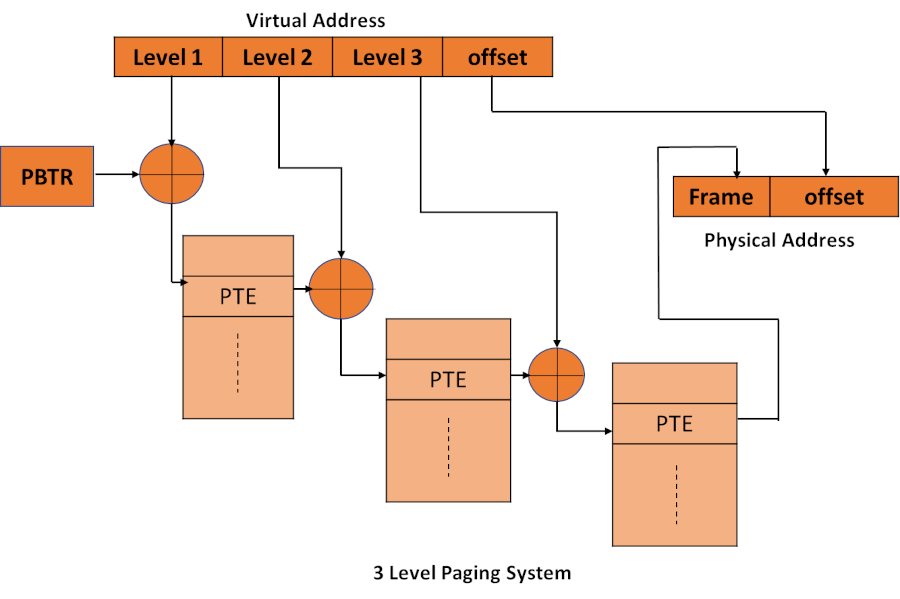
\includegraphics[scale=0.4]{./images/paging_03.jpeg}
      \end{figure}

    \begin{minipage}{\linewidth}
    \item Example of multi level page table.  \\

  \begin{myTableStyle}
    \begin{tabular}{ |m{4cm}|m{1cm}|m{5cm}| } \hline
        Page Size               &   \(2^{12}\) B  & offset bits = 12        \\ \hline
        Page Table Entry Size   &   \(2^{2}\)  B  &                         \\ \hline
        No of PTE in one page   &   \(2^{10}\) B  & offset bits for every level = 10        \\ \hline
        Physical Address Space  &   \(2^{44}\) B  & 32 + 12                 \\ \hline
        Logical Address Space   &   \(2^{32}\) B  & 10 + 10 + 12            \\ \hline
    \end{tabular}
  \end{myTableStyle}
  \vspace{0.08in}

    \begin{myTableStyle}
      \begin{tabular}{ |m{2cm}|m{2cm}|m{2cm}|m{2cm}|m{2cm}| } \hline
                  &  size           & total pages   & PTE         &  PT-size        \\ \hline
          Process &  \(2^{32}\) B   &  \(2^{20}\)   &  \(2^2\) B  &  \(2^{22}\) B   \\ \hline
          L-2     &  \(2^{22}\) B   &  \(2^{10}\)   &  \(2^2\) B  &  \(2^{12}\) B   \\ \hline
          L-1     &  \(2^{12}\) B   &  1            &  NA         &  NA             \\ \hline
      \end{tabular}
    \end{myTableStyle}
    \vspace{0.08in}

    \end{minipage}


    \begin{minipage}{\linewidth}
    \item Example of multi level page table.  \\

  \begin{myTableStyle}
    \begin{tabular}{ |m{4cm}|m{1cm}|m{5cm}| } \hline
        Page Size               &   \(2^{20}\) B  & offset bits = 20        \\ \hline
        Page Table Entry Size   &   \(2^{2}\)  B  &                         \\ \hline
        No of PTE in one page   &   \(2^{18}\) B  & offset bits for every level = 18        \\ \hline
        Physical Address Space  &                 &                          \\ \hline
        Logical Address Space   &   \(2^{64}\) B  & 8 + 18 + 18 + 20            \\ \hline
    \end{tabular}
  \end{myTableStyle}
  \vspace{0.08in}

    \begin{myTableStyle}
      \begin{tabular}{ |m{2cm}|m{2cm}|m{2cm}|m{2cm}|m{2cm}| } \hline
                  &  size           & total pages   & PTE         &  PT-size        \\ \hline
          Process &  \(2^{64}\) B   &  \(2^{44}\)   &  \(2^2\) B  &  \(2^{46}\) B   \\ \hline
          L-3     &  \(2^{46}\) B   &  \(2^{26}\)   &  \(2^2\) B  &  \(2^{28}\) B   \\ \hline
          L-2     &  \(2^{28}\) B   &  \(2^{8}\)    &  \(2^2\) B  &  \(2^{10}\) B   \\ \hline
          L-1     &  \(2^{10}\) B   &  1            &  NA         &  NA             \\ \hline
      \end{tabular}
    \end{myTableStyle}
    \vspace{0.08in}

    \end{minipage}


\end{enumerate}

% ----------------------------------------------------------------------------

% ----------------------------------------------------------------------------

% ----------------------------------------------------------------------------

% ----------------------------------------------------------------------------

% ----------------------------------------------------------------------------

% ----------------------------------------------------------------------------

% ----------------------------------------------------------------------------

% ----------------------------------------------------------------------------
